\documentclass[12pt, twoside]{article}
\usepackage[letterpaper, margin=1in, headsep=0.5in]{geometry}
\usepackage[english]{babel}
\usepackage[utf8]{inputenc}
\usepackage{amsmath}
\usepackage{amsfonts}
\usepackage{amssymb}
\usepackage{tikz}
\usetikzlibrary{quotes, angles}
\usepackage{graphicx}
%\usepackage{pgfplots}
%\pgfplotsset{width=10cm,compat=1.9}
%\usepgfplotslibrary{statistics}
%\usepackage{pgfplotstable}
%\usepackage{tkz-fct}
%\usepackage{venndiagram}

\usepackage{fancyhdr}
\pagestyle{fancy}
\fancyhf{}
\renewcommand{\headrulewidth}{0pt} % disable the underline of the header

\fancyhead[RE]{\thepage}
\fancyhead[RO]{\thepage \\ Name: \hspace{3cm}}
\fancyhead[L]{BECA / Dr. Huson / Geometry 10th Grade\\* Unit 1: Introduction to Geometry\\12 September 2019}

\begin{document}
\subsubsection*{1.6 Do Now: Angle Pairs}
  \vspace{0.5cm}
  \begin{enumerate}

  \item Complete the construction of an equilateral triangle with one side $\overline{RS}$. Fill in the blanks in the steps.
    \begin{enumerate}
      \item Given line segment $\overline{RS}$. \bigskip
      \item Construct a circle centered at point $R$ with radius $RS$.  \bigskip
      \item Construct a circle centered at point $\rule{2cm}{0.15mm}$  with radius $RS$. \bigskip
      \item Label the intersection of circle $R$ and $S$ as the point $T$. \bigskip
      \item Draw the line segment $\overline{RT}$ and the line segment  $\rule{2cm}{0.15mm}$.
      \bigskip
      \item $\triangle RST$ is an equilateral triangle.
    \end{enumerate}
    \vspace{8cm}
    \begin{center}
    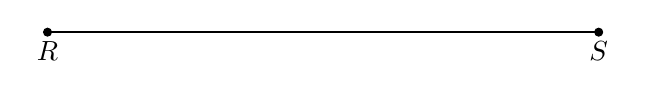
\begin{tikzpicture}
      \draw [-, thick] (0,0)--(7,0);
      \draw [fill] (0,0) circle [radius=0.05] node[below]{$R$};
      \draw [fill] (7,0) circle [radius=0.05] node[below]{$S$};
    \end{tikzpicture}
    \end{center}

\newpage
  \item Points that are all located on the same plane are $\rule{4cm}{0.15mm}$. \bigskip

  \item Given $\overline{ABC}$, $AB=3.8$, and $BC=1.7$.
  \begin{enumerate}
    \item Find ${AC}$.\\[1.5cm]
      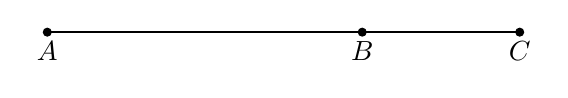
\begin{tikzpicture}
        \draw [-, thick] (1,0)--(7,0);
        \draw [fill] (1,0) circle [radius=0.05] node[below]{$A$};
        \draw [fill] (5,0) circle [radius=0.05] node[below]{$B$};
        \draw [fill] (7,0) circle [radius=0.05] node[below]{$C$};
      \end{tikzpicture} \vspace{2cm}
    \item The postulate used in this problem is the \rule{6cm}{0.15mm}.
  \end{enumerate}

  \item Given $\overleftrightarrow{MN}$ as shown on the number line. \\[20pt] % Midpoint
    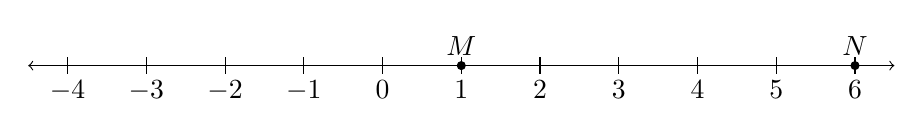
\begin{tikzpicture}
      \draw [<->] (-4.5,0)--(6.5,0);
      \foreach \x in {-4,...,6} %2 leading for diff!=1
        \draw[shift={(\x,0)},color=black] (0pt,-3pt) -- (0pt,3pt) node[below=5pt]  {$\x$};
        \draw [fill] (1,0) circle [radius=0.05] node[above] {$M$};
        \draw [fill] (6,0) circle [radius=0.05] node[above] {$N$};
    \end{tikzpicture} \\ \bigskip
    What is the distance on the number line between the points $M$ and $N$? \vspace{2cm}

  \item Given the situation in the diagram, answer each question. Circle True or False. \vspace{1cm}
      \begin{flushright}
      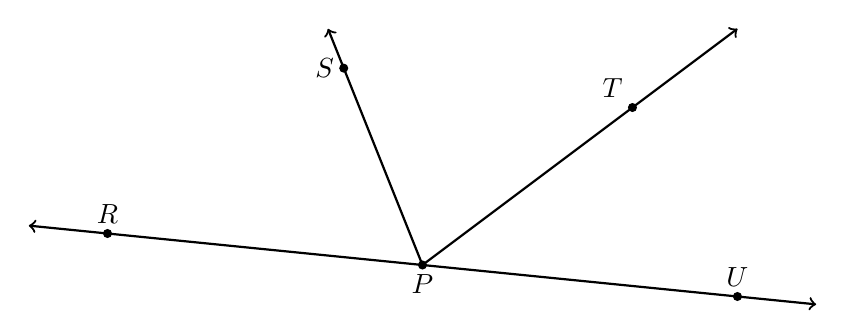
\begin{tikzpicture}[scale=1]
        \draw [->, thick] (0,0)--(4,3);
        \draw [<->, thick] (-5,.5)--(5,-.5);
        \draw [->, thick] (0,0)--(-1.2,3);
        \draw [fill] (-1,2.5) circle [radius=0.05] node[left ]{$S$};
        \draw [fill] (2.66666,2) circle [radius=0.05] node[above left ]{$T$};
        \draw [fill] (0,0) circle [radius=0.05] node[below]{$P$};
        \draw [fill] (4,-0.4) circle [radius=0.05] node[above]{$U$};
        \draw [fill] (-4,0.4) circle [radius=0.05] node[above]{$R$};
      \end{tikzpicture}
      \end{flushright}
    \begin{enumerate}
      \item True or False: $\overrightarrow{PR}$ and $\overrightarrow{UP}$ are opposite rays.\bigskip
      \item True or False: $\angle TPU$ is an obtuse angle.\bigskip
      \item True or False: $\angle RPS$ and $\angle TPU$ are vertical angles.\bigskip
      \item True or False: $\angle RPT$ and $\angle TPU$ are adjacent angles. \bigskip
    \end{enumerate}


  \end{enumerate}

\end{document}
